\hypertarget{_tsyg2004_8f}{
\section{/home/mgh/LanlGeoMag/libLanlGeoMag/Tsyg2004.f File Reference}
\label{_tsyg2004_8f}\index{/home/mgh/LanlGeoMag/libLanlGeoMag/Tsyg2004.f@{/home/mgh/LanlGeoMag/libLanlGeoMag/Tsyg2004.f}}
}
\subsection*{Functions}
\begin{CompactItemize}
\item 
subroutine \hyperlink{_tsyg2004_8f_76115f6519bc65ea6c916f3272219d4a}{T04S} (IOPT, PARMOD, PS, X, Y, Z, BX, BY, BZ)
\item 
subroutine \hyperlink{_tsyg2004_8f_f4e6ad8b8fa3f74e2914723b740c130c}{EXTERN} (IOPGEN, IOPT, IOPB, IOPR, A, NTOT,$\ast$PDYN, DST, BXIMF, BYIMF, BZIMF, W1, W2, W3, W4, W5, W6, PS, X, Y, Z,$\ast$BXCF, BYCF, BZCF, BXT1, BYT1, BZT1, BXT2, BYT2, BZT2,$\ast$BXSRC, BYSRC, BZSRC, BXPRC, BYPRC, BZPRC, BXR11, BYR11, BZR11,$\ast$BXR12, BYR12, BZR12, BXR21, BYR21, BZR21, BXR22, BYR22, BZR22, HXIMF,$\ast$HYIMF, HZIMF, BX, BY, BZ)
\item 
subroutine \hyperlink{_tsyg2004_8f_d52c74fa97a8f0a23954d670e0e0b84a}{SHLCAR3X3} (X, Y, Z, PS, BX, BY, BZ)
\item 
subroutine \hyperlink{_tsyg2004_8f_62fcead2ce484cd76fdc162bd2e72ca3}{DEFORMED} (IOPT, PS, X, Y, Z, BX1, BY1, BZ1, BX2, BY2, BZ2)
\item 
subroutine \hyperlink{_tsyg2004_8f_25094ad80471178e624b89c840009cc6}{WARPED} (IOPT, PS, X, Y, Z, BX1, BY1, BZ1, BX2, BY2, BZ2)
\item 
subroutine \hyperlink{_tsyg2004_8f_08d1be0e49f67539068d7f8dd74b4b9e}{UNWARPED} (IOPT, X, Y, Z, BX1, BY1, BZ1, BX2, BY2, BZ2)
\item 
subroutine \hyperlink{_tsyg2004_8f_23e0bc0f4d505d14f49527e132c8d7e3}{TAILDISK} (D0, DELTADX, DELTADY, X, Y, Z, BX, BY, BZ)
\item 
subroutine \hyperlink{_tsyg2004_8f_46ca699b5ea2961face078efbaa5da64}{SHLCAR5X5} (A, X, Y, Z, DSHIFT, HX, HY, HZ)
\item 
subroutine \hyperlink{_tsyg2004_8f_eb6fb8bb0214fdedda1df2ef2336c3fe}{BIRK\_\-TOT} (IOPB, PS, X, Y, Z, BX11, BY11, BZ11, BX12, BY12, BZ12,$\ast$BX21, BY21, BZ21, BX22, BY22, BZ22)
\item 
subroutine \hyperlink{_tsyg2004_8f_a74cccacc3c5e631324e705627f8ef28}{BIRK\_\-1N2} (NUMB, MODE, PS, X, Y, Z, BX, BY, BZ)
\item 
subroutine \hyperlink{_tsyg2004_8f_da6b1a3dc7523ce7bc09c55324951441}{TWOCONES} (A, X, Y, Z, BX, BY, BZ)
\item 
subroutine \hyperlink{_tsyg2004_8f_ab281013369e2f232027ff169264fd07}{ONE\_\-CONE} (A, X, Y, Z, BX, BY, BZ)
\item 
DOUBLE PRECISION \hyperlink{_tsyg2004_8f_a821422093810532210ff6f1aec0920d}{R\_\-S} (A, R, THETA)
\item 
DOUBLE PRECISION \hyperlink{_tsyg2004_8f_a12656461ac8bbe57d950d6788f8a70a}{THETA\_\-S} (A, R, THETA)
\item 
subroutine \hyperlink{_tsyg2004_8f_a235fc0d312a21adba2d5810919adca8}{FIALCOS} (R, THETA, PHI, BTHETA, BPHI, N, THETA0, DT)
\item 
subroutine \hyperlink{_tsyg2004_8f_a921f6b182c2c1697df43273aa36f99e}{BIRK\_\-SHL} (A, PS, X\_\-SC, X, Y, Z, BX, BY, BZ)
\item 
subroutine \hyperlink{_tsyg2004_8f_0d4d2f068a308fa1c6c4bb86fac16f9b}{FULL\_\-RC} (IOPR, PS, X, Y, Z, BXSRC, BYSRC, BZSRC, BXPRC, BYPRC,$\ast$BZPRC)
\item 
subroutine \hyperlink{_tsyg2004_8f_948852414e8750ea8068ebe4f3d03e96}{SRC\_\-PRC} (IOPR, SC\_\-SY, SC\_\-PR, PHI, PS, X, Y, Z, BXSRC, BYSRC,$\ast$BZSRC, BXPRC, BYPRC, BZPRC)
\item 
subroutine \hyperlink{_tsyg2004_8f_53c65a56be777ddfe059d5623b3ee80e}{RC\_\-SYMM} (X, Y, Z, BX, BY, BZ)
\item 
DOUBLE PRECISION \hyperlink{_tsyg2004_8f_6241cc7194479481c6845fe9216f73f9}{AP} (R, SINT, COST)
\item 
subroutine \hyperlink{_tsyg2004_8f_e5d2a482ea368498294fcc6bedc734ad}{PRC\_\-SYMM} (X, Y, Z, BX, BY, BZ)
\item 
DOUBLE PRECISION \hyperlink{_tsyg2004_8f_d97fe9780c85165cf3d5efc106ad9f0e}{APPRC} (R, SINT, COST)
\item 
subroutine \hyperlink{_tsyg2004_8f_00310f7aecb95af18d5be726d529f907}{PRC\_\-QUAD} (X, Y, Z, BX, BY, BZ)
\item 
DOUBLE PRECISION \hyperlink{_tsyg2004_8f_d87c020522fe895268a9166c3f8292f6}{BR\_\-PRC\_\-Q} (R, SINT, COST)
\item 
DOUBLE PRECISION \hyperlink{_tsyg2004_8f_dbd25510c3ba667598e7c14abcc5b786}{BT\_\-PRC\_\-Q} (R, SINT, COST)
\item 
subroutine \hyperlink{_tsyg2004_8f_8d9b5c31c4fb074683c40c0fa923c3a2}{FFS} (A, A0, DA, F, FA, FS)
\item 
subroutine \hyperlink{_tsyg2004_8f_f5b31c6f54b60f926656e483aa50ebac}{RC\_\-SHIELD} (A, PS, X\_\-SC, X, Y, Z, BX, BY, BZ)
\item 
subroutine \hyperlink{_tsyg2004_8f_b2b4bf9a582d902f19522d4db9af8f34}{DIPOLE} (PS, X, Y, Z, BX, BY, BZ)
\end{CompactItemize}


\subsection{Function Documentation}
\hypertarget{_tsyg2004_8f_76115f6519bc65ea6c916f3272219d4a}{
\index{Tsyg2004.f@{Tsyg2004.f}!T04S@{T04S}}
\index{T04S@{T04S}!Tsyg2004.f@{Tsyg2004.f}}
\subsubsection[{T04S}]{\setlength{\rightskip}{0pt plus 5cm}subroutine T04S (IOPT, \/  REAL$\ast$8,dimension(10) {\em PARMOD}, \/  REAL$\ast$8 {\em PS}, \/  REAL$\ast$8 {\em X}, \/  REAL$\ast$8 {\em Y}, \/  REAL$\ast$8 {\em Z}, \/  REAL$\ast$8 {\em BX}, \/  REAL$\ast$8 {\em BY}, \/  REAL$\ast$8 {\em BZ})}}
\label{_tsyg2004_8f_76115f6519bc65ea6c916f3272219d4a}




Definition at line 5 of file Tsyg2004.f.

Here is the call graph for this function:\nopagebreak
\begin{figure}[H]
\begin{center}
\leavevmode
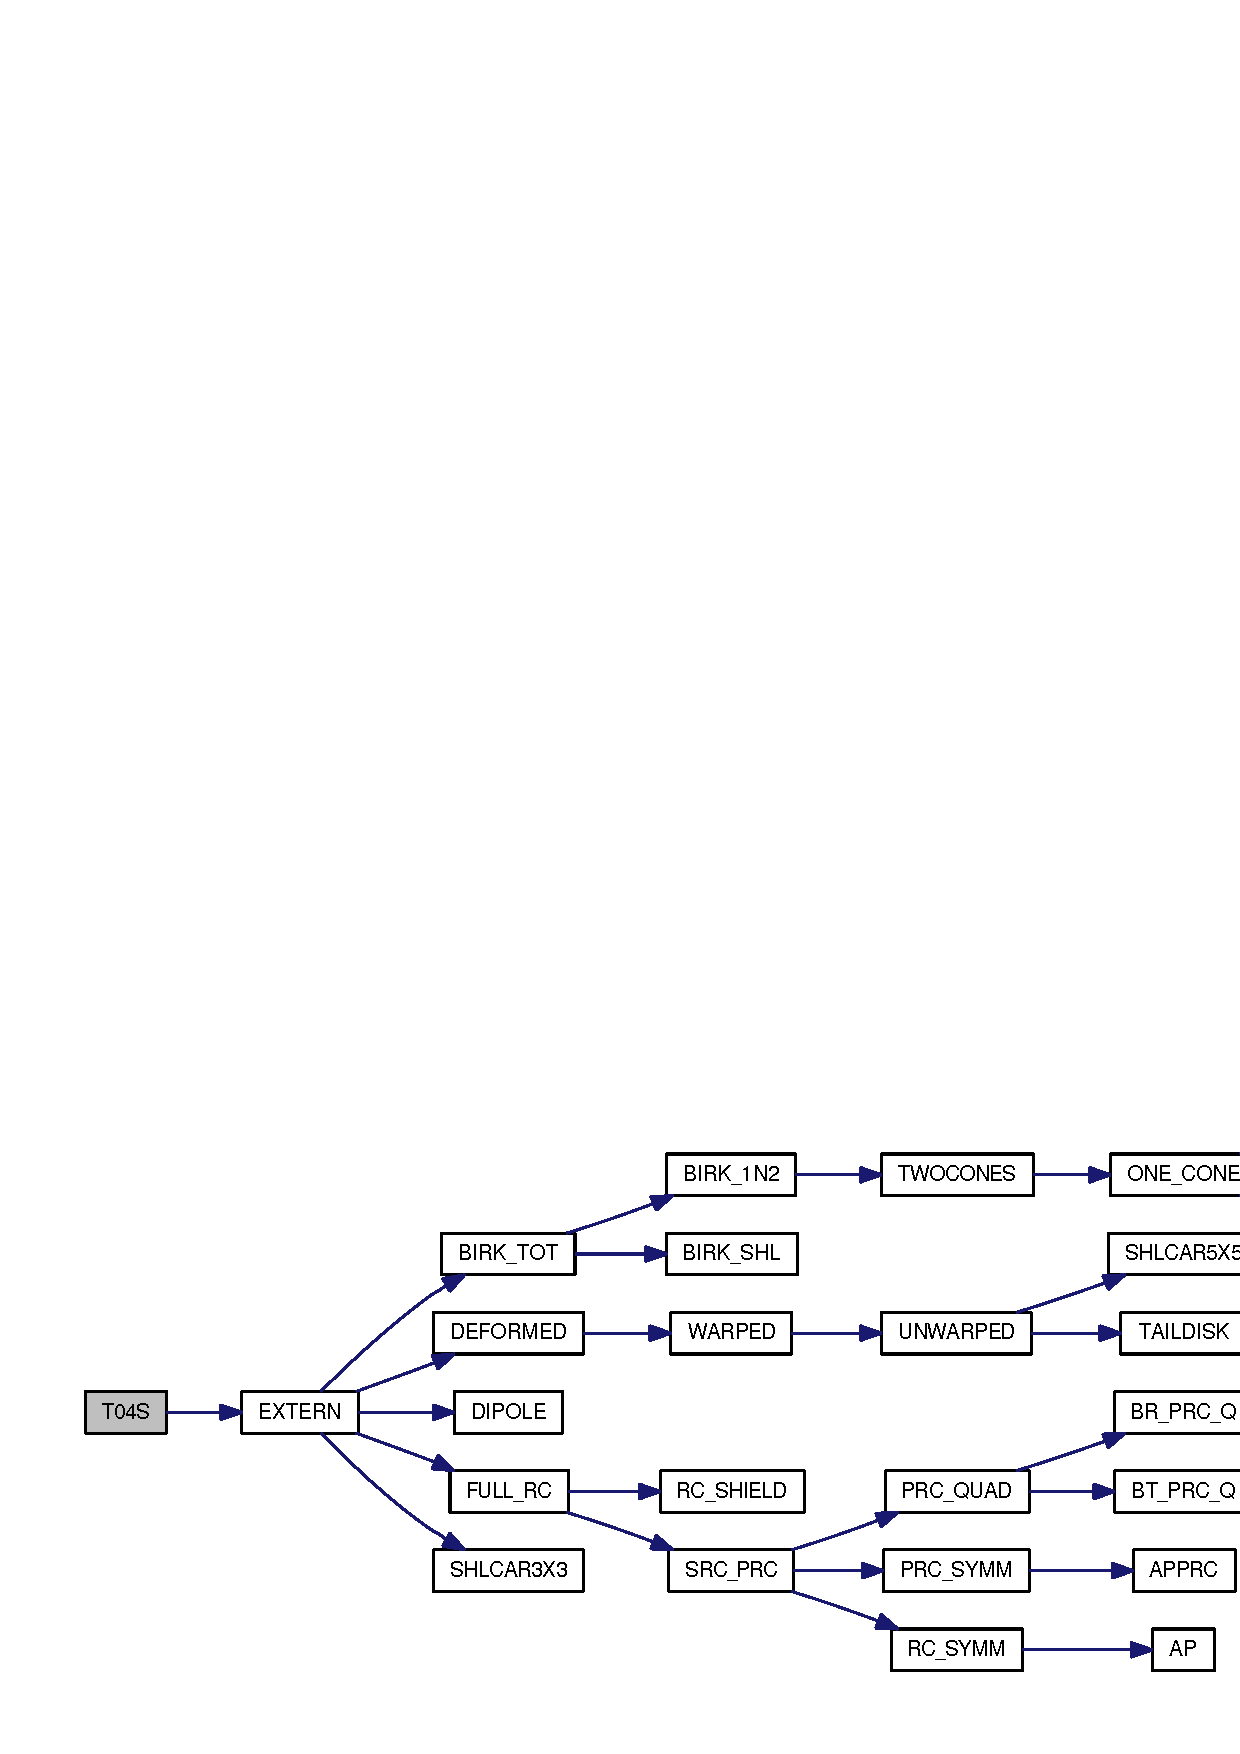
\includegraphics[width=352pt]{_tsyg2004_8f_76115f6519bc65ea6c916f3272219d4a_cgraph}
\end{center}
\end{figure}
\hypertarget{_tsyg2004_8f_f4e6ad8b8fa3f74e2914723b740c130c}{
\index{Tsyg2004.f@{Tsyg2004.f}!EXTERN@{EXTERN}}
\index{EXTERN@{EXTERN}!Tsyg2004.f@{Tsyg2004.f}}
\subsubsection[{EXTERN}]{\setlength{\rightskip}{0pt plus 5cm}subroutine EXTERN (IOPGEN, \/  IOPT, \/  IOPB, \/  IOPR, \/  A, \/  NTOT, \/  $\ast$ {\em PDYN}, \/  DST, \/  BXIMF, \/  BYIMF, \/  BZIMF, \/  W1, \/  W2, \/  W3, \/  W4, \/  W5, \/  W6, \/  PS, \/  X, \/  Y, \/  Z, \/  $\ast$ {\em BXCF}, \/  BYCF, \/  BZCF, \/  BXT1, \/  BYT1, \/  BZT1, \/  BXT2, \/  BYT2, \/  BZT2, \/  $\ast$ {\em BXSRC}, \/  BYSRC, \/  BZSRC, \/  BXPRC, \/  BYPRC, \/  BZPRC, \/  BXR11, \/  BYR11, \/  BZR11, \/  $\ast$ {\em BXR12}, \/  BYR12, \/  BZR12, \/  BXR21, \/  BYR21, \/  BZR21, \/  BXR22, \/  BYR22, \/  BZR22, \/  HXIMF, \/  $\ast$ {\em HYIMF}, \/  HZIMF, \/  BX, \/  BY, \/  BZ)}}
\label{_tsyg2004_8f_f4e6ad8b8fa3f74e2914723b740c130c}




Definition at line 123 of file Tsyg2004.f.

Here is the call graph for this function:\nopagebreak
\begin{figure}[H]
\begin{center}
\leavevmode
\includegraphics[width=314pt]{_tsyg2004_8f_f4e6ad8b8fa3f74e2914723b740c130c_cgraph}
\end{center}
\end{figure}


Here is the caller graph for this function:\nopagebreak
\begin{figure}[H]
\begin{center}
\leavevmode
\includegraphics[width=88pt]{_tsyg2004_8f_f4e6ad8b8fa3f74e2914723b740c130c_icgraph}
\end{center}
\end{figure}
\hypertarget{_tsyg2004_8f_d52c74fa97a8f0a23954d670e0e0b84a}{
\index{Tsyg2004.f@{Tsyg2004.f}!SHLCAR3X3@{SHLCAR3X3}}
\index{SHLCAR3X3@{SHLCAR3X3}!Tsyg2004.f@{Tsyg2004.f}}
\subsubsection[{SHLCAR3X3}]{\setlength{\rightskip}{0pt plus 5cm}subroutine SHLCAR3X3 (X, \/  Y, \/  Z, \/  PS, \/  BX, \/  BY, \/  BZ)}}
\label{_tsyg2004_8f_d52c74fa97a8f0a23954d670e0e0b84a}




Definition at line 362 of file Tsyg2004.f.\hypertarget{_tsyg2004_8f_62fcead2ce484cd76fdc162bd2e72ca3}{
\index{Tsyg2004.f@{Tsyg2004.f}!DEFORMED@{DEFORMED}}
\index{DEFORMED@{DEFORMED}!Tsyg2004.f@{Tsyg2004.f}}
\subsubsection[{DEFORMED}]{\setlength{\rightskip}{0pt plus 5cm}subroutine DEFORMED (IOPT, \/  PS, \/  X, \/  Y, \/  Z, \/  BX1, \/  BY1, \/  BZ1, \/  BX2, \/  BY2, \/  BZ2)}}
\label{_tsyg2004_8f_62fcead2ce484cd76fdc162bd2e72ca3}




Definition at line 709 of file Tsyg2004.f.

Here is the call graph for this function:\nopagebreak
\begin{figure}[H]
\begin{center}
\leavevmode
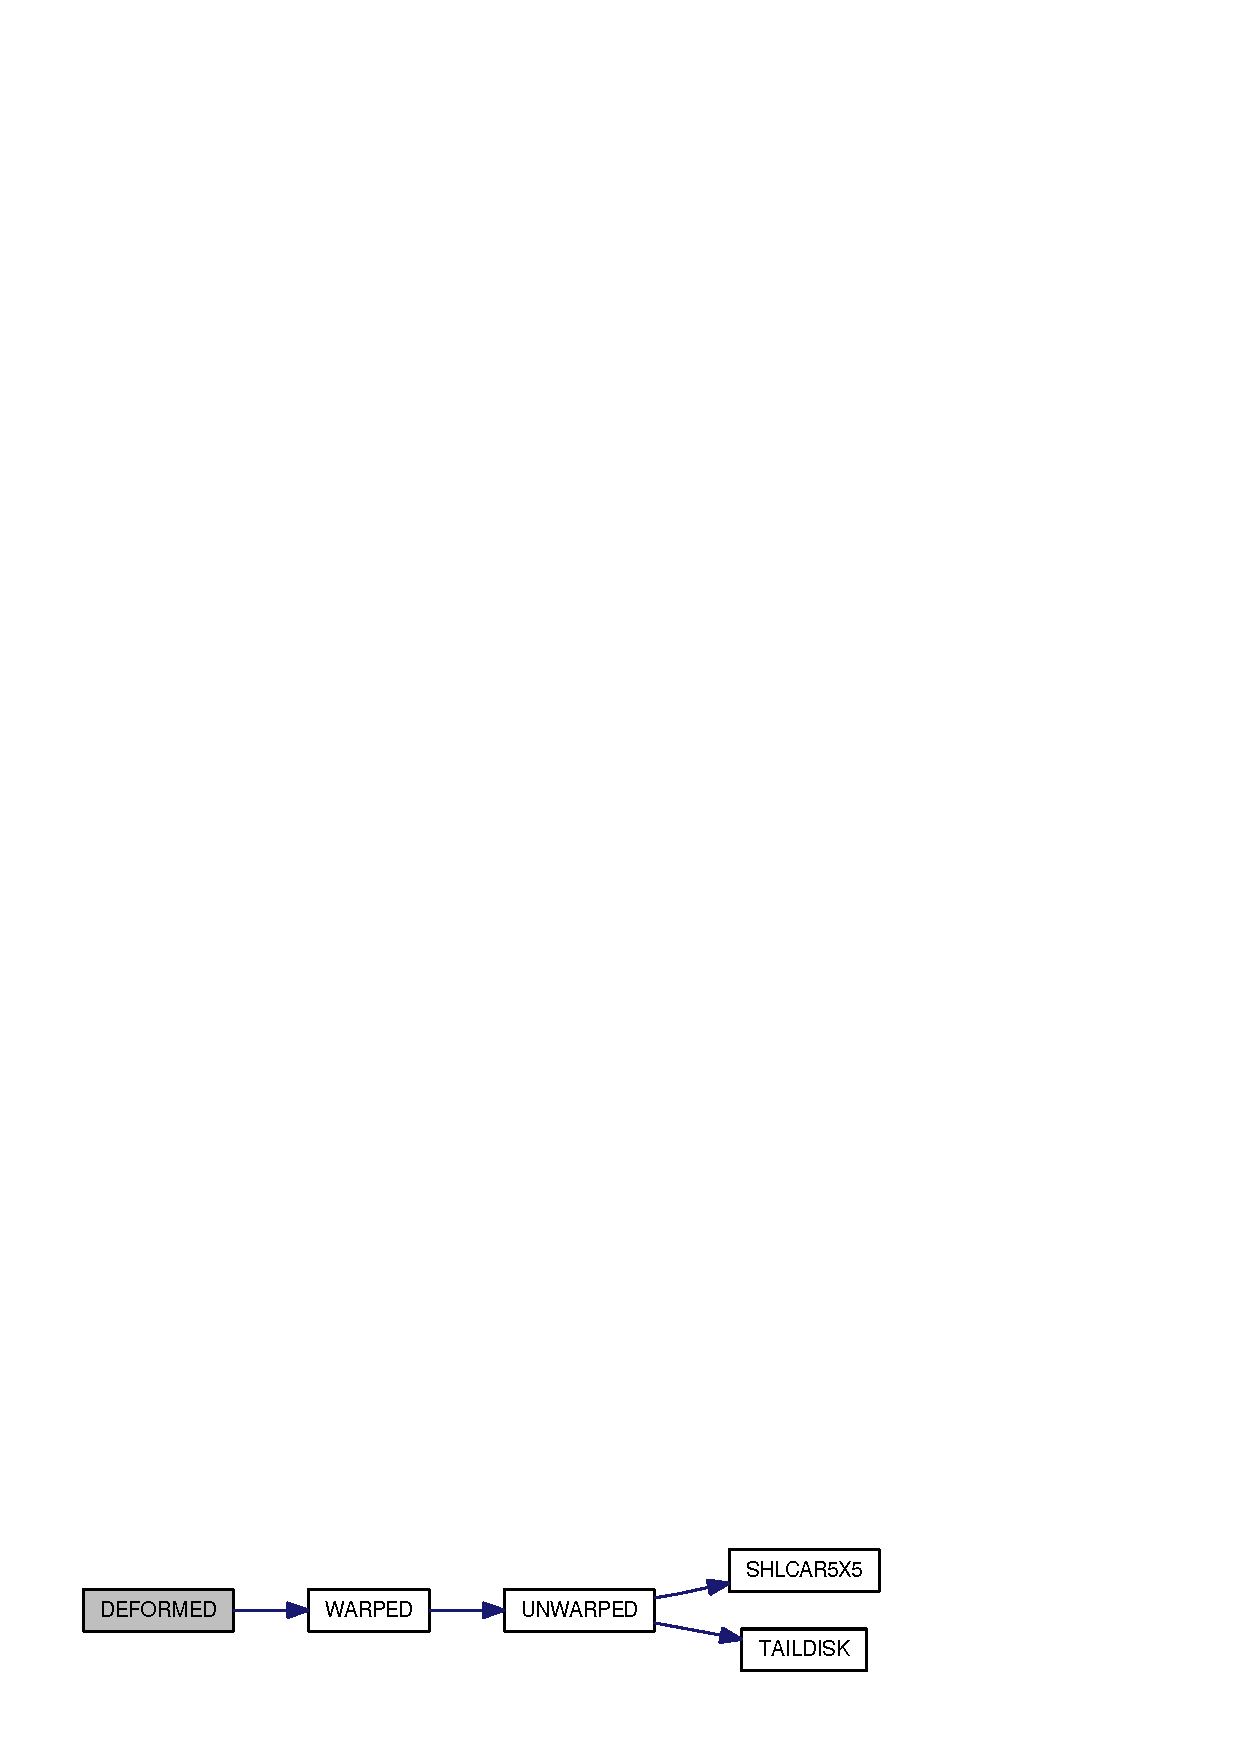
\includegraphics[width=213pt]{_tsyg2004_8f_62fcead2ce484cd76fdc162bd2e72ca3_cgraph}
\end{center}
\end{figure}
\hypertarget{_tsyg2004_8f_25094ad80471178e624b89c840009cc6}{
\index{Tsyg2004.f@{Tsyg2004.f}!WARPED@{WARPED}}
\index{WARPED@{WARPED}!Tsyg2004.f@{Tsyg2004.f}}
\subsubsection[{WARPED}]{\setlength{\rightskip}{0pt plus 5cm}subroutine WARPED (IOPT, \/  PS, \/  X, \/  Y, \/  Z, \/  BX1, \/  BY1, \/  BZ1, \/  BX2, \/  BY2, \/  BZ2)}}
\label{_tsyg2004_8f_25094ad80471178e624b89c840009cc6}




Definition at line 779 of file Tsyg2004.f.

Here is the call graph for this function:\nopagebreak
\begin{figure}[H]
\begin{center}
\leavevmode
\includegraphics[width=159pt]{_tsyg2004_8f_25094ad80471178e624b89c840009cc6_cgraph}
\end{center}
\end{figure}
\hypertarget{_tsyg2004_8f_08d1be0e49f67539068d7f8dd74b4b9e}{
\index{Tsyg2004.f@{Tsyg2004.f}!UNWARPED@{UNWARPED}}
\index{UNWARPED@{UNWARPED}!Tsyg2004.f@{Tsyg2004.f}}
\subsubsection[{UNWARPED}]{\setlength{\rightskip}{0pt plus 5cm}subroutine UNWARPED (IOPT, \/  X, \/  Y, \/  Z, \/  BX1, \/  BY1, \/  BZ1, \/  BX2, \/  BY2, \/  BZ2)}}
\label{_tsyg2004_8f_08d1be0e49f67539068d7f8dd74b4b9e}




Definition at line 852 of file Tsyg2004.f.

Here is the call graph for this function:\nopagebreak
\begin{figure}[H]
\begin{center}
\leavevmode
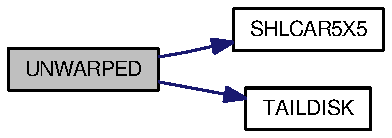
\includegraphics[width=112pt]{_tsyg2004_8f_08d1be0e49f67539068d7f8dd74b4b9e_cgraph}
\end{center}
\end{figure}
\hypertarget{_tsyg2004_8f_23e0bc0f4d505d14f49527e132c8d7e3}{
\index{Tsyg2004.f@{Tsyg2004.f}!TAILDISK@{TAILDISK}}
\index{TAILDISK@{TAILDISK}!Tsyg2004.f@{Tsyg2004.f}}
\subsubsection[{TAILDISK}]{\setlength{\rightskip}{0pt plus 5cm}subroutine TAILDISK (D0, \/  DELTADX, \/  DELTADY, \/  X, \/  Y, \/  Z, \/  BX, \/  BY, \/  BZ)}}
\label{_tsyg2004_8f_23e0bc0f4d505d14f49527e132c8d7e3}




Definition at line 991 of file Tsyg2004.f.\hypertarget{_tsyg2004_8f_46ca699b5ea2961face078efbaa5da64}{
\index{Tsyg2004.f@{Tsyg2004.f}!SHLCAR5X5@{SHLCAR5X5}}
\index{SHLCAR5X5@{SHLCAR5X5}!Tsyg2004.f@{Tsyg2004.f}}
\subsubsection[{SHLCAR5X5}]{\setlength{\rightskip}{0pt plus 5cm}subroutine SHLCAR5X5 (A, \/  X, \/  Y, \/  Z, \/  DSHIFT, \/  HX, \/  HY, \/  HZ)}}
\label{_tsyg2004_8f_46ca699b5ea2961face078efbaa5da64}




Definition at line 1082 of file Tsyg2004.f.\hypertarget{_tsyg2004_8f_eb6fb8bb0214fdedda1df2ef2336c3fe}{
\index{Tsyg2004.f@{Tsyg2004.f}!BIRK\_\-TOT@{BIRK\_\-TOT}}
\index{BIRK\_\-TOT@{BIRK\_\-TOT}!Tsyg2004.f@{Tsyg2004.f}}
\subsubsection[{BIRK\_\-TOT}]{\setlength{\rightskip}{0pt plus 5cm}subroutine BIRK\_\-TOT (IOPB, \/  PS, \/  X, \/  Y, \/  Z, \/  BX11, \/  BY11, \/  BZ11, \/  BX12, \/  BY12, \/  BZ12, \/  $\ast$ {\em BX21}, \/  BY21, \/  BZ21, \/  BX22, \/  BY22, \/  BZ22)}}
\label{_tsyg2004_8f_eb6fb8bb0214fdedda1df2ef2336c3fe}




Definition at line 1137 of file Tsyg2004.f.

Here is the call graph for this function:\nopagebreak
\begin{figure}[H]
\begin{center}
\leavevmode
\includegraphics[width=260pt]{_tsyg2004_8f_eb6fb8bb0214fdedda1df2ef2336c3fe_cgraph}
\end{center}
\end{figure}
\hypertarget{_tsyg2004_8f_a74cccacc3c5e631324e705627f8ef28}{
\index{Tsyg2004.f@{Tsyg2004.f}!BIRK\_\-1N2@{BIRK\_\-1N2}}
\index{BIRK\_\-1N2@{BIRK\_\-1N2}!Tsyg2004.f@{Tsyg2004.f}}
\subsubsection[{BIRK\_\-1N2}]{\setlength{\rightskip}{0pt plus 5cm}subroutine BIRK\_\-1N2 (NUMB, \/  MODE, \/  PS, \/  X, \/  Y, \/  Z, \/  BX, \/  BY, \/  BZ)}}
\label{_tsyg2004_8f_a74cccacc3c5e631324e705627f8ef28}




Definition at line 1363 of file Tsyg2004.f.

Here is the call graph for this function:\nopagebreak
\begin{figure}[H]
\begin{center}
\leavevmode
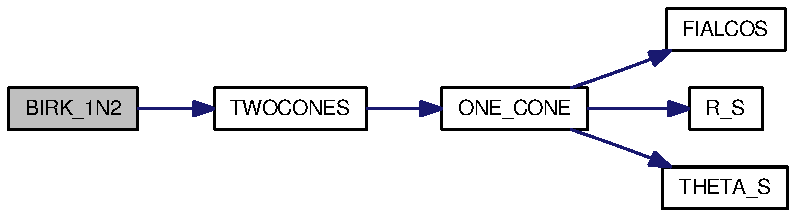
\includegraphics[width=209pt]{_tsyg2004_8f_a74cccacc3c5e631324e705627f8ef28_cgraph}
\end{center}
\end{figure}
\hypertarget{_tsyg2004_8f_da6b1a3dc7523ce7bc09c55324951441}{
\index{Tsyg2004.f@{Tsyg2004.f}!TWOCONES@{TWOCONES}}
\index{TWOCONES@{TWOCONES}!Tsyg2004.f@{Tsyg2004.f}}
\subsubsection[{TWOCONES}]{\setlength{\rightskip}{0pt plus 5cm}subroutine TWOCONES (A, \/  X, \/  Y, \/  Z, \/  BX, \/  BY, \/  BZ)}}
\label{_tsyg2004_8f_da6b1a3dc7523ce7bc09c55324951441}




Definition at line 1528 of file Tsyg2004.f.

Here is the call graph for this function:\nopagebreak
\begin{figure}[H]
\begin{center}
\leavevmode
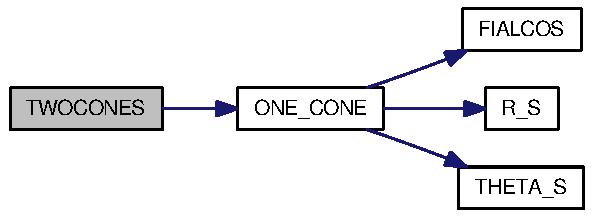
\includegraphics[width=160pt]{_tsyg2004_8f_da6b1a3dc7523ce7bc09c55324951441_cgraph}
\end{center}
\end{figure}
\hypertarget{_tsyg2004_8f_ab281013369e2f232027ff169264fd07}{
\index{Tsyg2004.f@{Tsyg2004.f}!ONE\_\-CONE@{ONE\_\-CONE}}
\index{ONE\_\-CONE@{ONE\_\-CONE}!Tsyg2004.f@{Tsyg2004.f}}
\subsubsection[{ONE\_\-CONE}]{\setlength{\rightskip}{0pt plus 5cm}subroutine ONE\_\-CONE (A, \/  X, \/  Y, \/  Z, \/  BX, \/  BY, \/  BZ)}}
\label{_tsyg2004_8f_ab281013369e2f232027ff169264fd07}




Definition at line 1548 of file Tsyg2004.f.

Here is the call graph for this function:\nopagebreak
\begin{figure}[H]
\begin{center}
\leavevmode
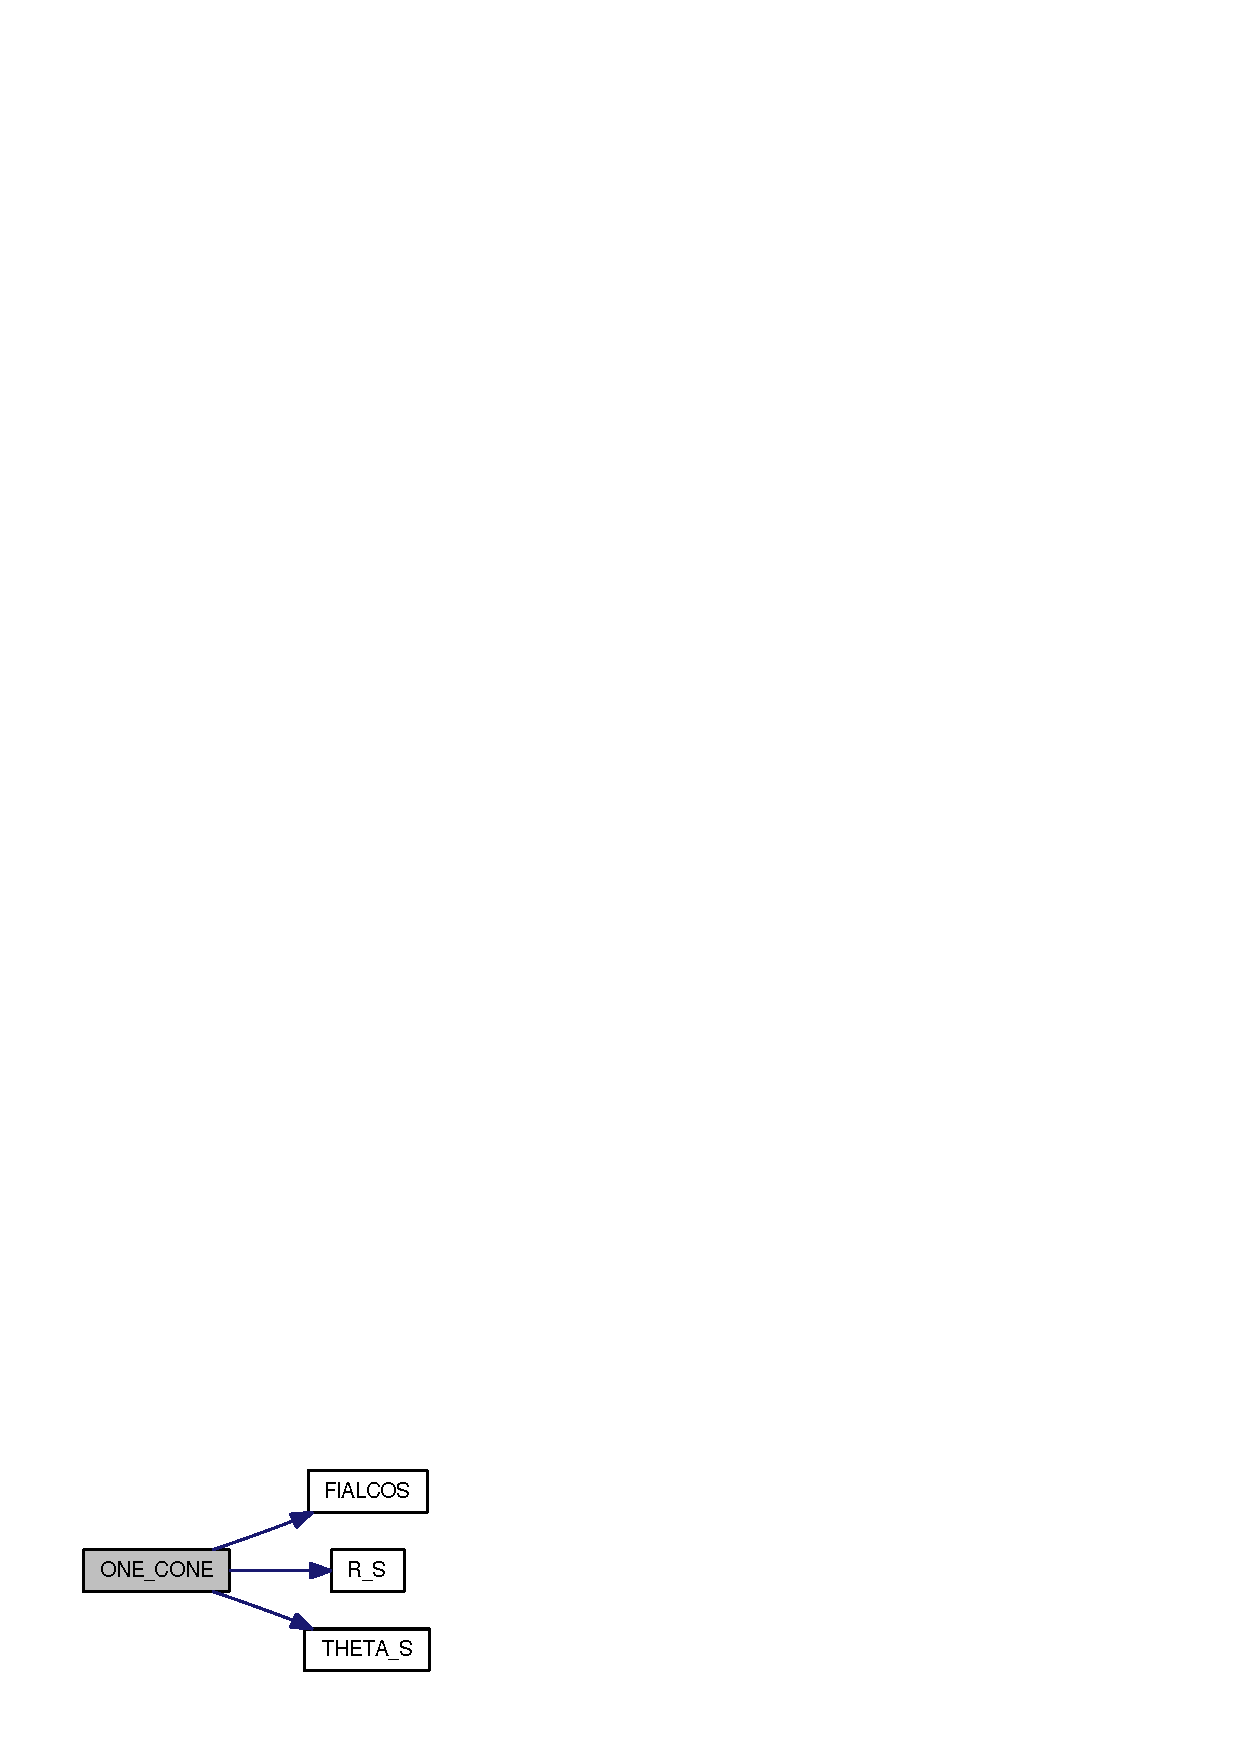
\includegraphics[width=105pt]{_tsyg2004_8f_ab281013369e2f232027ff169264fd07_cgraph}
\end{center}
\end{figure}
\hypertarget{_tsyg2004_8f_a821422093810532210ff6f1aec0920d}{
\index{Tsyg2004.f@{Tsyg2004.f}!R\_\-S@{R\_\-S}}
\index{R\_\-S@{R\_\-S}!Tsyg2004.f@{Tsyg2004.f}}
\subsubsection[{R\_\-S}]{\setlength{\rightskip}{0pt plus 5cm}DOUBLE PRECISION R\_\-S (A, \/  R, \/  THETA)}}
\label{_tsyg2004_8f_a821422093810532210ff6f1aec0920d}




Definition at line 1611 of file Tsyg2004.f.

Here is the call graph for this function:\nopagebreak
\begin{figure}[H]
\begin{center}
\leavevmode
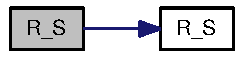
\includegraphics[width=76pt]{_tsyg2004_8f_a821422093810532210ff6f1aec0920d_cgraph}
\end{center}
\end{figure}
\hypertarget{_tsyg2004_8f_a12656461ac8bbe57d950d6788f8a70a}{
\index{Tsyg2004.f@{Tsyg2004.f}!THETA\_\-S@{THETA\_\-S}}
\index{THETA\_\-S@{THETA\_\-S}!Tsyg2004.f@{Tsyg2004.f}}
\subsubsection[{THETA\_\-S}]{\setlength{\rightskip}{0pt plus 5cm}DOUBLE PRECISION THETA\_\-S (A, \/  R, \/  THETA)}}
\label{_tsyg2004_8f_a12656461ac8bbe57d950d6788f8a70a}




Definition at line 1626 of file Tsyg2004.f.

Here is the call graph for this function:\nopagebreak
\begin{figure}[H]
\begin{center}
\leavevmode
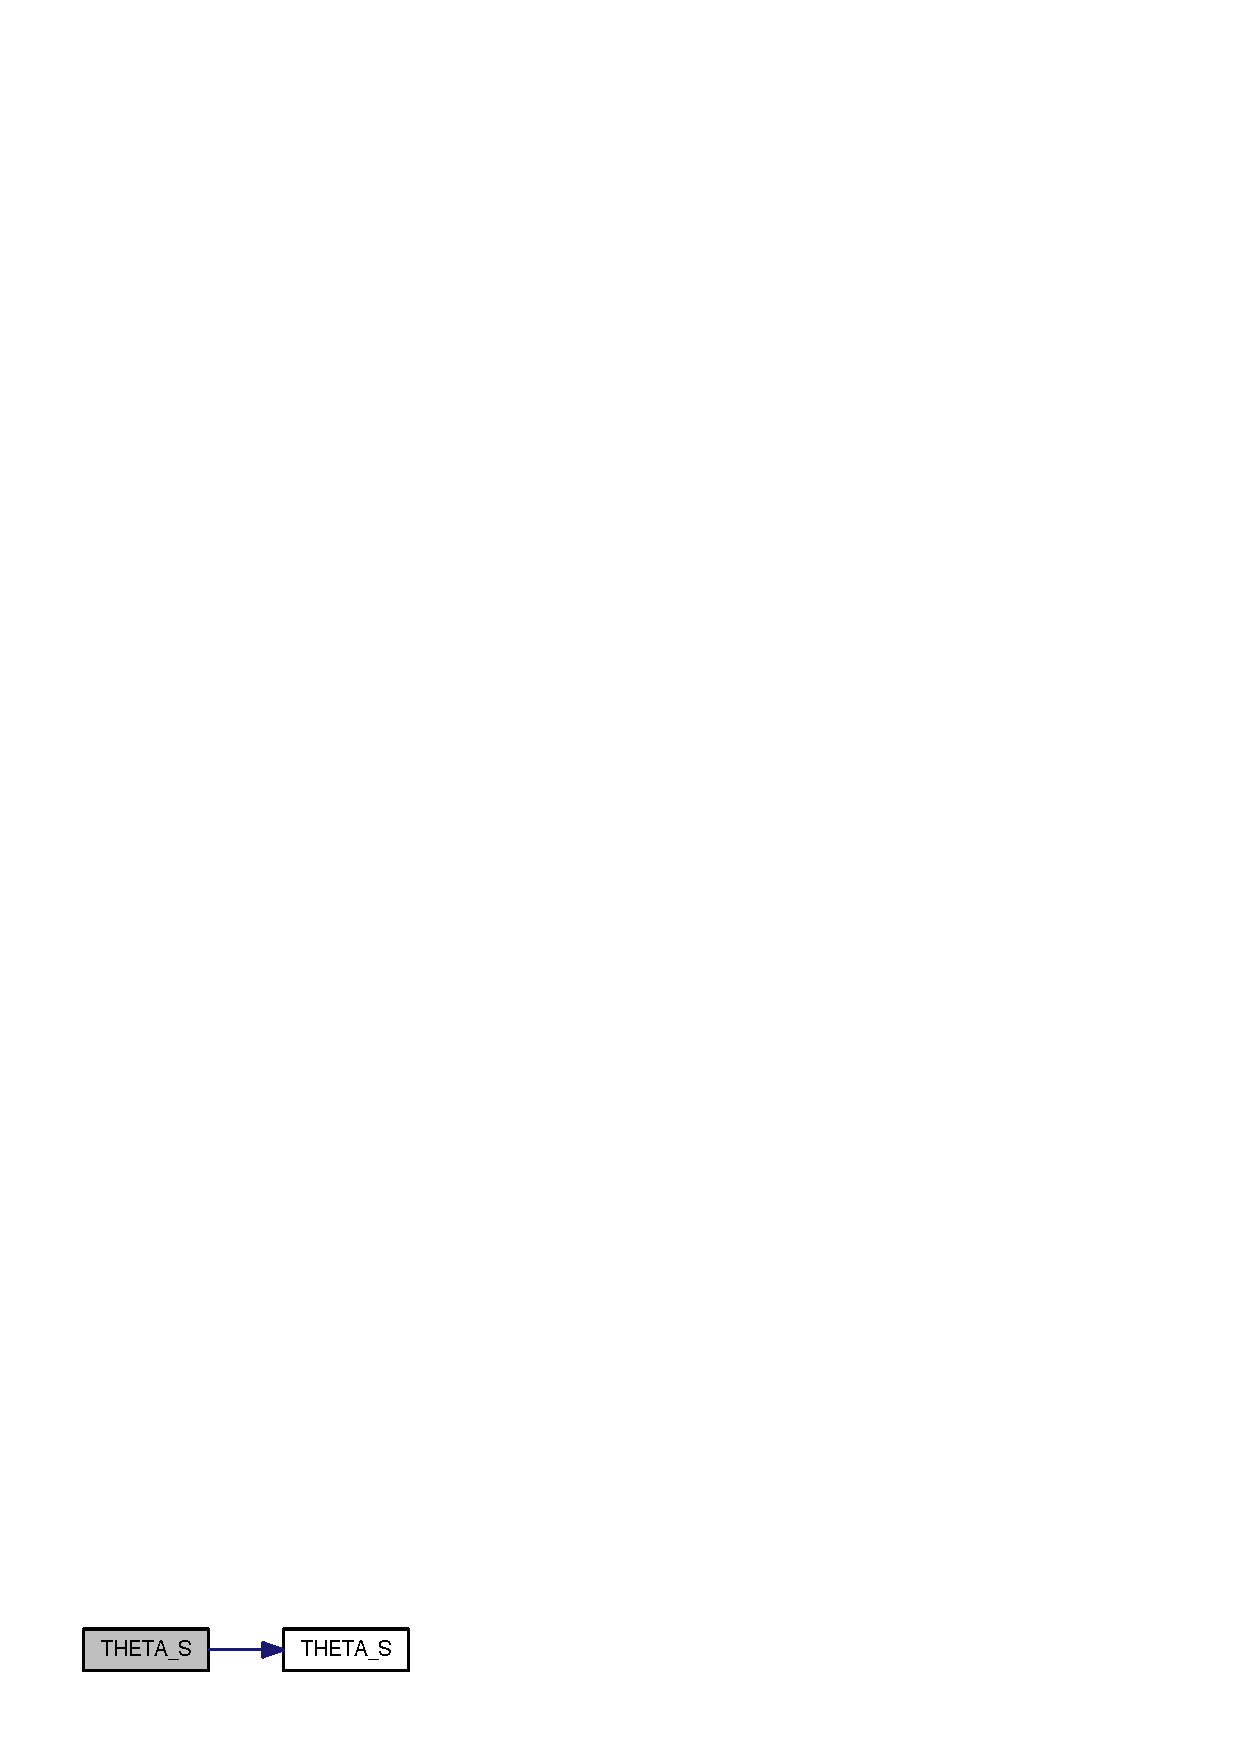
\includegraphics[width=100pt]{_tsyg2004_8f_a12656461ac8bbe57d950d6788f8a70a_cgraph}
\end{center}
\end{figure}
\hypertarget{_tsyg2004_8f_a235fc0d312a21adba2d5810919adca8}{
\index{Tsyg2004.f@{Tsyg2004.f}!FIALCOS@{FIALCOS}}
\index{FIALCOS@{FIALCOS}!Tsyg2004.f@{Tsyg2004.f}}
\subsubsection[{FIALCOS}]{\setlength{\rightskip}{0pt plus 5cm}subroutine FIALCOS (R, \/  THETA, \/  PHI, \/  BTHETA, \/  BPHI, \/  N, \/  THETA0, \/  DT)}}
\label{_tsyg2004_8f_a235fc0d312a21adba2d5810919adca8}




Definition at line 1641 of file Tsyg2004.f.\hypertarget{_tsyg2004_8f_a921f6b182c2c1697df43273aa36f99e}{
\index{Tsyg2004.f@{Tsyg2004.f}!BIRK\_\-SHL@{BIRK\_\-SHL}}
\index{BIRK\_\-SHL@{BIRK\_\-SHL}!Tsyg2004.f@{Tsyg2004.f}}
\subsubsection[{BIRK\_\-SHL}]{\setlength{\rightskip}{0pt plus 5cm}subroutine BIRK\_\-SHL (A, \/  PS, \/  X\_\-SC, \/  X, \/  Y, \/  Z, \/  BX, \/  BY, \/  BZ)}}
\label{_tsyg2004_8f_a921f6b182c2c1697df43273aa36f99e}




Definition at line 1719 of file Tsyg2004.f.\hypertarget{_tsyg2004_8f_0d4d2f068a308fa1c6c4bb86fac16f9b}{
\index{Tsyg2004.f@{Tsyg2004.f}!FULL\_\-RC@{FULL\_\-RC}}
\index{FULL\_\-RC@{FULL\_\-RC}!Tsyg2004.f@{Tsyg2004.f}}
\subsubsection[{FULL\_\-RC}]{\setlength{\rightskip}{0pt plus 5cm}subroutine FULL\_\-RC (IOPR, \/  PS, \/  X, \/  Y, \/  Z, \/  BXSRC, \/  BYSRC, \/  BZSRC, \/  BXPRC, \/  BYPRC, \/  $\ast$ {\em BZPRC})}}
\label{_tsyg2004_8f_0d4d2f068a308fa1c6c4bb86fac16f9b}




Definition at line 1856 of file Tsyg2004.f.

Here is the call graph for this function:\nopagebreak
\begin{figure}[H]
\begin{center}
\leavevmode
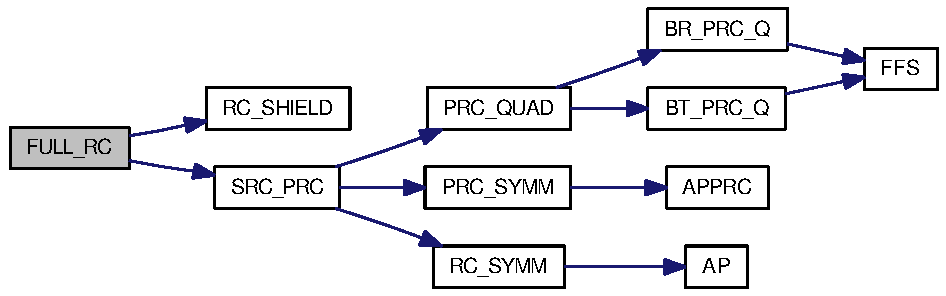
\includegraphics[width=245pt]{_tsyg2004_8f_0d4d2f068a308fa1c6c4bb86fac16f9b_cgraph}
\end{center}
\end{figure}
\hypertarget{_tsyg2004_8f_948852414e8750ea8068ebe4f3d03e96}{
\index{Tsyg2004.f@{Tsyg2004.f}!SRC\_\-PRC@{SRC\_\-PRC}}
\index{SRC\_\-PRC@{SRC\_\-PRC}!Tsyg2004.f@{Tsyg2004.f}}
\subsubsection[{SRC\_\-PRC}]{\setlength{\rightskip}{0pt plus 5cm}subroutine SRC\_\-PRC (IOPR, \/  SC\_\-SY, \/  SC\_\-PR, \/  PHI, \/  PS, \/  X, \/  Y, \/  Z, \/  BXSRC, \/  BYSRC, \/  $\ast$ {\em BZSRC}, \/  BXPRC, \/  BYPRC, \/  BZPRC)}}
\label{_tsyg2004_8f_948852414e8750ea8068ebe4f3d03e96}




Definition at line 1995 of file Tsyg2004.f.

Here is the call graph for this function:\nopagebreak
\begin{figure}[H]
\begin{center}
\leavevmode
\includegraphics[width=193pt]{_tsyg2004_8f_948852414e8750ea8068ebe4f3d03e96_cgraph}
\end{center}
\end{figure}
\hypertarget{_tsyg2004_8f_53c65a56be777ddfe059d5623b3ee80e}{
\index{Tsyg2004.f@{Tsyg2004.f}!RC\_\-SYMM@{RC\_\-SYMM}}
\index{RC\_\-SYMM@{RC\_\-SYMM}!Tsyg2004.f@{Tsyg2004.f}}
\subsubsection[{RC\_\-SYMM}]{\setlength{\rightskip}{0pt plus 5cm}subroutine RC\_\-SYMM (X, \/  Y, \/  Z, \/  BX, \/  BY, \/  BZ)}}
\label{_tsyg2004_8f_53c65a56be777ddfe059d5623b3ee80e}




Definition at line 2080 of file Tsyg2004.f.

Here is the call graph for this function:\nopagebreak
\begin{figure}[H]
\begin{center}
\leavevmode
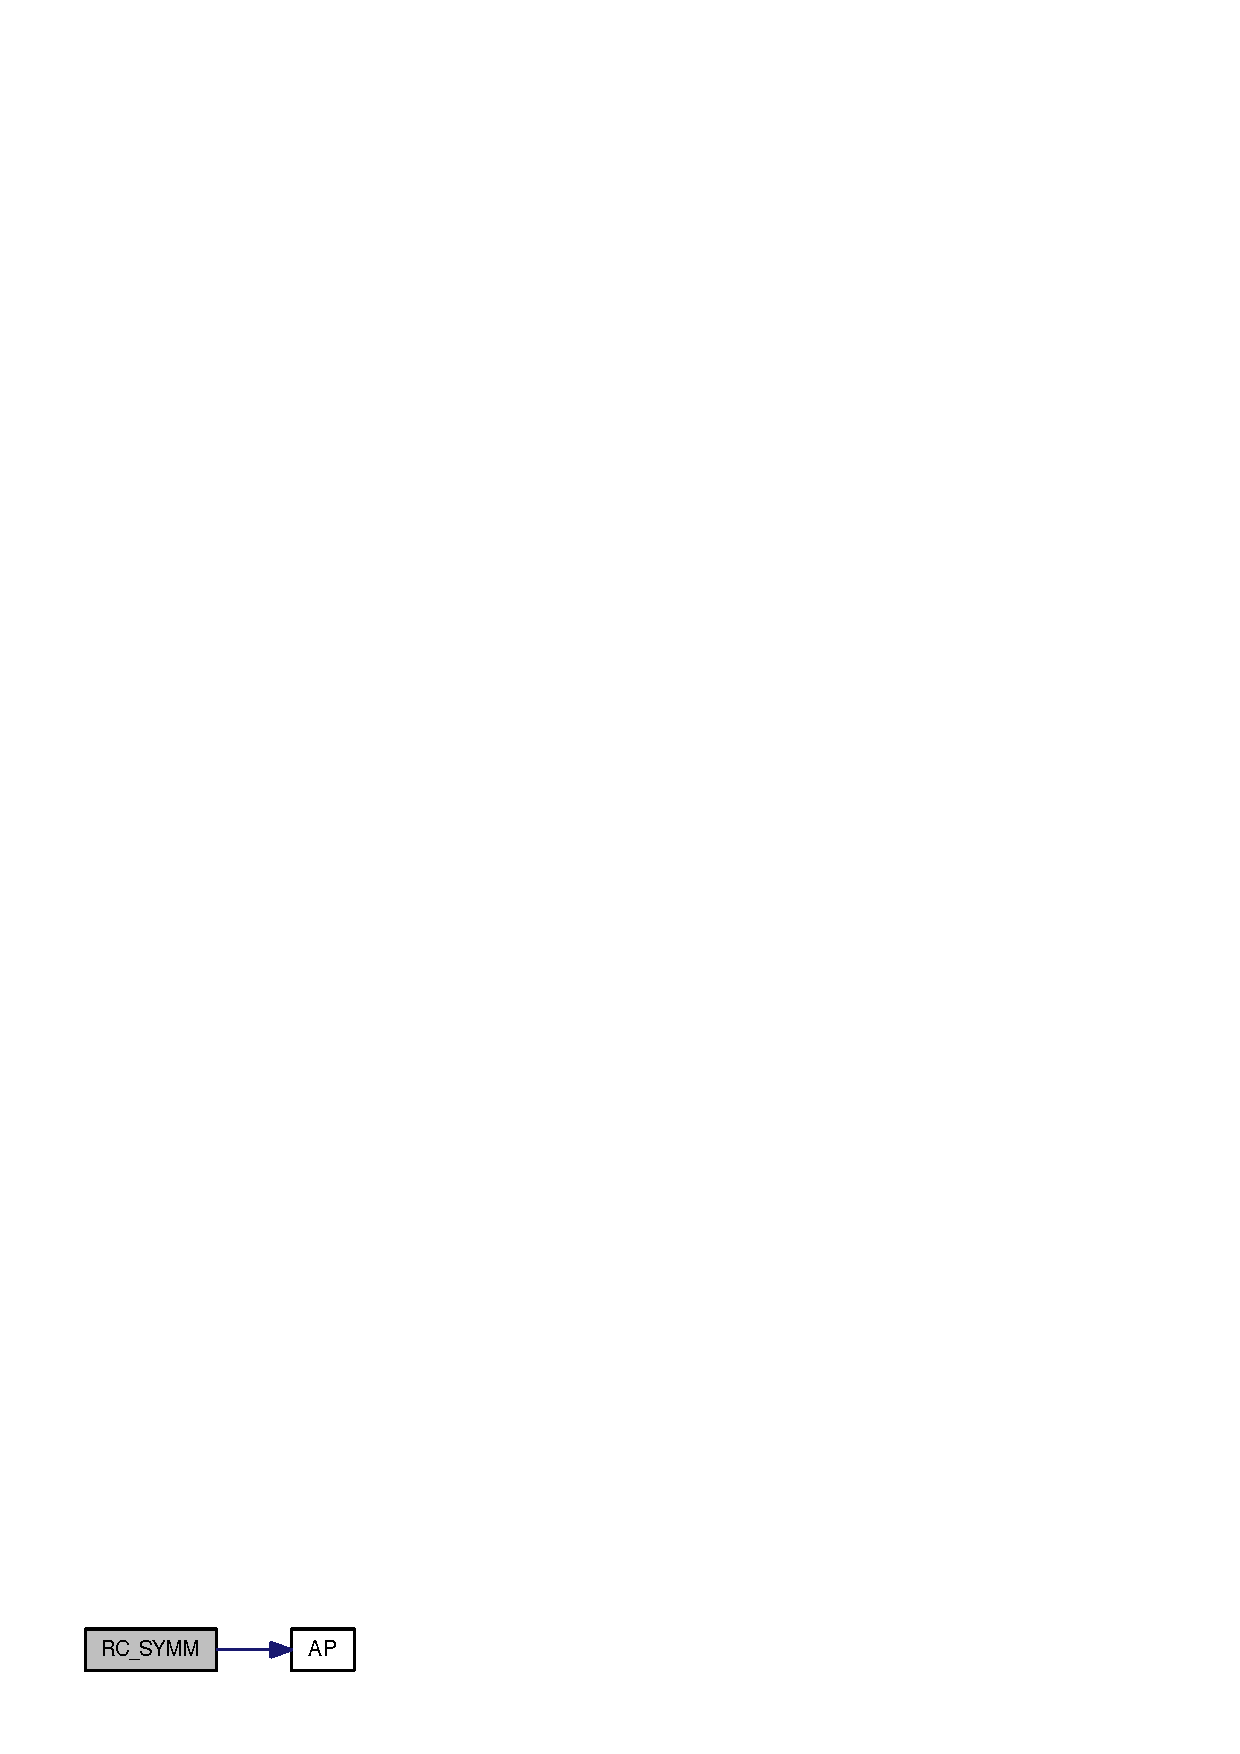
\includegraphics[width=87pt]{_tsyg2004_8f_53c65a56be777ddfe059d5623b3ee80e_cgraph}
\end{center}
\end{figure}
\hypertarget{_tsyg2004_8f_6241cc7194479481c6845fe9216f73f9}{
\index{Tsyg2004.f@{Tsyg2004.f}!AP@{AP}}
\index{AP@{AP}!Tsyg2004.f@{Tsyg2004.f}}
\subsubsection[{AP}]{\setlength{\rightskip}{0pt plus 5cm}DOUBLE PRECISION AP (R, \/  SINT, \/  COST)}}
\label{_tsyg2004_8f_6241cc7194479481c6845fe9216f73f9}




Definition at line 2126 of file Tsyg2004.f.

Here is the call graph for this function:\nopagebreak
\begin{figure}[H]
\begin{center}
\leavevmode
\includegraphics[width=70pt]{_tsyg2004_8f_6241cc7194479481c6845fe9216f73f9_cgraph}
\end{center}
\end{figure}
\hypertarget{_tsyg2004_8f_e5d2a482ea368498294fcc6bedc734ad}{
\index{Tsyg2004.f@{Tsyg2004.f}!PRC\_\-SYMM@{PRC\_\-SYMM}}
\index{PRC\_\-SYMM@{PRC\_\-SYMM}!Tsyg2004.f@{Tsyg2004.f}}
\subsubsection[{PRC\_\-SYMM}]{\setlength{\rightskip}{0pt plus 5cm}subroutine PRC\_\-SYMM (X, \/  Y, \/  Z, \/  BX, \/  BY, \/  BZ)}}
\label{_tsyg2004_8f_e5d2a482ea368498294fcc6bedc734ad}




Definition at line 2245 of file Tsyg2004.f.

Here is the call graph for this function:\nopagebreak
\begin{figure}[H]
\begin{center}
\leavevmode
\includegraphics[width=100pt]{_tsyg2004_8f_e5d2a482ea368498294fcc6bedc734ad_cgraph}
\end{center}
\end{figure}
\hypertarget{_tsyg2004_8f_d97fe9780c85165cf3d5efc106ad9f0e}{
\index{Tsyg2004.f@{Tsyg2004.f}!APPRC@{APPRC}}
\index{APPRC@{APPRC}!Tsyg2004.f@{Tsyg2004.f}}
\subsubsection[{APPRC}]{\setlength{\rightskip}{0pt plus 5cm}DOUBLE PRECISION APPRC (R, \/  SINT, \/  COST)}}
\label{_tsyg2004_8f_d97fe9780c85165cf3d5efc106ad9f0e}




Definition at line 2291 of file Tsyg2004.f.

Here is the call graph for this function:\nopagebreak
\begin{figure}[H]
\begin{center}
\leavevmode
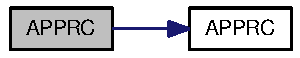
\includegraphics[width=90pt]{_tsyg2004_8f_d97fe9780c85165cf3d5efc106ad9f0e_cgraph}
\end{center}
\end{figure}
\hypertarget{_tsyg2004_8f_00310f7aecb95af18d5be726d529f907}{
\index{Tsyg2004.f@{Tsyg2004.f}!PRC\_\-QUAD@{PRC\_\-QUAD}}
\index{PRC\_\-QUAD@{PRC\_\-QUAD}!Tsyg2004.f@{Tsyg2004.f}}
\subsubsection[{PRC\_\-QUAD}]{\setlength{\rightskip}{0pt plus 5cm}subroutine PRC\_\-QUAD (X, \/  Y, \/  Z, \/  BX, \/  BY, \/  BZ)}}
\label{_tsyg2004_8f_00310f7aecb95af18d5be726d529f907}




Definition at line 2413 of file Tsyg2004.f.

Here is the call graph for this function:\nopagebreak
\begin{figure}[H]
\begin{center}
\leavevmode
\includegraphics[width=145pt]{_tsyg2004_8f_00310f7aecb95af18d5be726d529f907_cgraph}
\end{center}
\end{figure}
\hypertarget{_tsyg2004_8f_d87c020522fe895268a9166c3f8292f6}{
\index{Tsyg2004.f@{Tsyg2004.f}!BR\_\-PRC\_\-Q@{BR\_\-PRC\_\-Q}}
\index{BR\_\-PRC\_\-Q@{BR\_\-PRC\_\-Q}!Tsyg2004.f@{Tsyg2004.f}}
\subsubsection[{BR\_\-PRC\_\-Q}]{\setlength{\rightskip}{0pt plus 5cm}DOUBLE PRECISION BR\_\-PRC\_\-Q (R, \/  SINT, \/  COST)}}
\label{_tsyg2004_8f_d87c020522fe895268a9166c3f8292f6}




Definition at line 2470 of file Tsyg2004.f.

Here is the call graph for this function:\nopagebreak
\begin{figure}[H]
\begin{center}
\leavevmode
\includegraphics[width=144pt]{_tsyg2004_8f_d87c020522fe895268a9166c3f8292f6_cgraph}
\end{center}
\end{figure}
\hypertarget{_tsyg2004_8f_dbd25510c3ba667598e7c14abcc5b786}{
\index{Tsyg2004.f@{Tsyg2004.f}!BT\_\-PRC\_\-Q@{BT\_\-PRC\_\-Q}}
\index{BT\_\-PRC\_\-Q@{BT\_\-PRC\_\-Q}!Tsyg2004.f@{Tsyg2004.f}}
\subsubsection[{BT\_\-PRC\_\-Q}]{\setlength{\rightskip}{0pt plus 5cm}DOUBLE PRECISION BT\_\-PRC\_\-Q (R, \/  SINT, \/  COST)}}
\label{_tsyg2004_8f_dbd25510c3ba667598e7c14abcc5b786}




Definition at line 2544 of file Tsyg2004.f.

Here is the call graph for this function:\nopagebreak
\begin{figure}[H]
\begin{center}
\leavevmode
\includegraphics[width=91pt]{_tsyg2004_8f_dbd25510c3ba667598e7c14abcc5b786_cgraph}
\end{center}
\end{figure}
\hypertarget{_tsyg2004_8f_8d9b5c31c4fb074683c40c0fa923c3a2}{
\index{Tsyg2004.f@{Tsyg2004.f}!FFS@{FFS}}
\index{FFS@{FFS}!Tsyg2004.f@{Tsyg2004.f}}
\subsubsection[{FFS}]{\setlength{\rightskip}{0pt plus 5cm}subroutine FFS (A, \/  A0, \/  DA, \/  F, \/  FA, \/  FS)}}
\label{_tsyg2004_8f_8d9b5c31c4fb074683c40c0fa923c3a2}




Definition at line 2607 of file Tsyg2004.f.

Here is the call graph for this function:\nopagebreak
\begin{figure}[H]
\begin{center}
\leavevmode
\includegraphics[width=127pt]{_tsyg2004_8f_8d9b5c31c4fb074683c40c0fa923c3a2_cgraph}
\end{center}
\end{figure}
\hypertarget{_tsyg2004_8f_f5b31c6f54b60f926656e483aa50ebac}{
\index{Tsyg2004.f@{Tsyg2004.f}!RC\_\-SHIELD@{RC\_\-SHIELD}}
\index{RC\_\-SHIELD@{RC\_\-SHIELD}!Tsyg2004.f@{Tsyg2004.f}}
\subsubsection[{RC\_\-SHIELD}]{\setlength{\rightskip}{0pt plus 5cm}subroutine RC\_\-SHIELD (A, \/  PS, \/  X\_\-SC, \/  X, \/  Y, \/  Z, \/  BX, \/  BY, \/  BZ)}}
\label{_tsyg2004_8f_f5b31c6f54b60f926656e483aa50ebac}




Definition at line 2622 of file Tsyg2004.f.\hypertarget{_tsyg2004_8f_b2b4bf9a582d902f19522d4db9af8f34}{
\index{Tsyg2004.f@{Tsyg2004.f}!DIPOLE@{DIPOLE}}
\index{DIPOLE@{DIPOLE}!Tsyg2004.f@{Tsyg2004.f}}
\subsubsection[{DIPOLE}]{\setlength{\rightskip}{0pt plus 5cm}subroutine DIPOLE (PS, \/  X, \/  Y, \/  Z, \/  BX, \/  BY, \/  BZ)}}
\label{_tsyg2004_8f_b2b4bf9a582d902f19522d4db9af8f34}




Definition at line 2760 of file Tsyg2004.f.